\documentclass[11pt,a4paper]{article}
\usepackage[left=2.5cm,right=2cm, bottom=2cm]{geometry}
\usepackage[utf8]{inputenc}
\usepackage{amsmath}
\usepackage{amsfonts}
\usepackage{amssymb}
\usepackage{amsfonts}
\usepackage{amsmath}
\usepackage{graphicx}
\usepackage{subfigure}
\usepackage{color}
\usepackage{abstract}
\usepackage{float}
\usepackage[toc,page]{appendix}
\usepackage{hyperref}
\usepackage{fancyhdr}
\usepackage{algorithm} 
\usepackage{algpseudocode} 
\usepackage{listings}
\usepackage{xcolor} % for setting colors
% set the default code style
\lstset{
	frame=tb, % draw a frame at the top and bottom of the code block
	tabsize=4, % tab space width
	showstringspaces=false, % don't mark spaces in strings
	numbers=left, % display line numbers on the left
	commentstyle=\color{green}, % comment color
	keywordstyle=\color{blue}, % keyword color
	stringstyle=\color{red} % string color
}

\pagestyle{fancy}
\fancyhf{}
\rhead{\today}
\lhead{\bfseries Alexander Leitner 01525882}
\rfoot{}



\begin{document}
\begin{center}
	\fontsize{24pt}{10pt}\selectfont
	\textsc{\textbf{Computational Science on Many-Core Architectures  Exercise 2}}
\end{center}
\section*{Example 1 Basic Cuda}
\subsection*{a)}
Seven different array length from $N = 10,100,1000,...10^7$ and its time for Malloc and Free.
\begin{figure}[H]
	\centering
	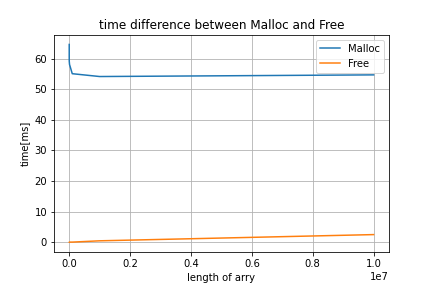
\includegraphics[width=0.50\textwidth]{Bilder/time_difference_between_Malloc_and_Free.png}
	\caption{5 turn}
\end{figure}
I run the code seven times and document the time results.
\begin{lstlisting}[language=C++, caption={code for a)}]
timer.reset();
// Allocate device memory and copy host data over
cudaMalloc(&d_x, N*sizeof(double)); 
cudaMalloc(&d_y, N*sizeof(double));
printf("a) cudaMalloc_initTime: %g[ms] N = %d\n", 1000*timer.get(),N);
cudaDeviceSynchronize();
timer.reset();
cudaFree(d_x);
cudaFree(d_y);
printf("a) cudaFree_initTime: %g[ms] N = %d\n", 1000*timer.get(),N);
\end{lstlisting}
\end{document}